\documentclass[conference]{IEEEtran}
\IEEEoverridecommandlockouts

% --- Encoding and fonts ---
\usepackage[T1]{fontenc}
\usepackage[utf8]{inputenc}

% --- Layout ---
\usepackage{microtype}

% --- Math ---
\usepackage{amsmath}
\usepackage{amssymb}
\usepackage{amsfonts}

% --- Figures and tables ---
\usepackage{graphicx}
\usepackage{array}
\usepackage{tabularx}
\usepackage{booktabs}
\usepackage{pgfplots}
\pgfplotsset{compat=1.18}
\usepackage{stfloats}
\usepackage{placeins}
\usepackage{float}
\usepackage{textcomp}
\usepackage{xcolor}
\newcolumntype{L}{>{\raggedright\arraybackslash}X}

\setlength{\dblfloatsep}{8pt plus 2pt minus 2pt}
\setlength{\dbltextfloatsep}{8pt plus 2pt minus 2pt}
\setcounter{topnumber}{4}
\setcounter{dbltopnumber}{4}
\setcounter{totalnumber}{6}
\renewcommand{\topfraction}{0.95}
\renewcommand{\dbltopfraction}{0.95}
\renewcommand{\textfraction}{0.05}
\renewcommand{\floatpagefraction}{0.7}
\renewcommand{\dblfloatpagefraction}{0.7}
\raggedbottom

\makeatletter
\setlength{\@fptop}{0pt}
\setlength{\@fpsep}{8pt plus 1pt minus 1pt}
\setlength{\@fpbot}{0pt plus 1fil}
\setlength{\@dblfptop}{0pt}
\setlength{\@dblfpsep}{8pt plus 1pt minus 1pt}
\setlength{\@dblfpbot}{0pt plus 1fil}
\makeatother

% --- Bibliography ---
\usepackage[backend=biber,style=ieee,sorting=none]{biblatex}
\addbibresource{bibliography.bib}
\renewcommand*{\bibfont}{\footnotesize}

% --- Links ---
\usepackage{xurl}
\usepackage[hidelinks]{hyperref}
\usepackage{cleveref}

\pgfplotsset{
  ieee common/.style={
    width=0.92\linewidth,
    height=4.4cm,
    ylabel style={font=\small},
    xlabel style={font=\small},
    xtick=data,
    axis on top,
    ymajorgrids=true,
    grid style={gray!25},
    tick label style={font=\scriptsize},
    legend style={
      at={(0.5,-0.22)},
      anchor=north,
      legend columns=2,
      font=\scriptsize,
      draw=black!45,
    },
    legend cell align=left,
  },
  ieee bars/.style={
    ieee common,
    ybar,
    bar width=7pt,
    enlarge x limits=0.25,
  },
  ieee lines/.style={
    ieee common,
    enlarge x limits=0.15,
    mark=*,
    mark size=1.6pt,
  }
}

% Draft marker. Delete each boxed note before the final submission.
\newcommand{\writer}[2]{%
  \par\medskip
  \noindent\fcolorbox{black}{yellow!25}{%
    \parbox{\dimexpr\linewidth-2\fboxsep-2\fboxrule\relax}{%
      \raggedright\textbf{WRITE THIS SECTION: #1.}\\[2pt]
      #2%
    }%
  }%
  \par\medskip
}

\begin{document}

\title{Caching Finite-Field Arithmetic\\for Determinant Evaluation}

\author{%
\IEEEauthorblockN{Jacob Nance}
\and
\IEEEauthorblockN{Fernanda Gonzalez}
\and
\IEEEauthorblockN{Francisco Chagua}
\and
\IEEEauthorblockN{Nicholas Hooper}
\and
\IEEEauthorblockN{Nicholas Johnson}
\and
\IEEEauthorblockN{Mohamed Konsowa}
}

\maketitle

\begin{abstract}
Matrix entries in this program are elements of the finite field of order \(11^3 = 1331\).
Each arithmetic operation reduces a polynomial modulo a fixed irreducible, so a determinant repeats the same products and sums many times.
The finite-field element type was replaced by a drop-in version that fills addition, multiplication, and reciprocal tables once and reuses them.
On one AMD Ryzen 9 7900X thread, the cached arithmetic was about five times faster than the original polynomial arithmetic at \(64 \times 64\) and at \(256 \times 256\).
The tables cost about 159\,MB and made the cached run slower for an \(8 \times 8\) matrix.
A blocked PLU determinant over MPI is implemented and not yet timed against the cached sequential determinant.
\end{abstract}

\section{Introduction}
\label{sec:introduction}

\writer{Whole group}{%
Describe the program: \(C = AB\) over the field of order \(11^3\), then \(\det(A)\), \(\det(B)\), and \(\det(C)\), with the check \(\det(C) = \det(A)\det(B)\).
State the three questions the assignment asks: which class was cached, how runtime and memory changed, and at what size MPI beats the cached sequential determinant.}

\section{Dependency Chain}
\label{sec:chain}

The driver links two libraries.
\texttt{algebra::matrices} stores the entries and implements matrix multiplication and row swaps.
\texttt{algebra::finite\_fields} supplies the entry type.
The driver fixes that type as \(\mathtt{FiniteField}\langle 11,3\rangle\), so every entry is an element of a degree-3 extension of the prime field \(\mathbb{F}_{11}\) \cite{russell2026fields,russell2026matrices}.
Polynomial arithmetic used by the field lives in a third library, pulled in by the finite-field package.
The matrices never reduce polynomials themselves.
They call \texttt{add}, \texttt{multiply}, \texttt{negate}, and \texttt{reciprocal} on the element type.

That split is why the finite-field element is the class to cache.
A change inside the element type is visible to multiplication and to elimination without editing the matrix templates or the driver.
The irreducible modulus stays the one chosen by the field's deterministic search.
On the profiled build the modulus was \(x^3 + x + 4\).

The sequential driver still computes \(C = AB\) with the library matrix product, then runs Gaussian elimination with partial pivoting for \(\det(A)\), \(\det(B)\), and \(\det(C)\).
The elimination is local to the driver.
It is the same algorithm for the original field and the cached field, so a timing difference between those two builds is a difference in element arithmetic.

\section{Cached Field Arithmetic}
\label{sec:cache}

Arithmetic in a finite field is limited to a small set of results determined by the field's cardinality \(q\).
For addition and multiplication, this requires up to \(q^2\) entries in each cache.
The reciprocal cache is smaller, with at most \(q\) entries.
Division does not require a separate cache because it is implemented as multiplication by the reciprocal.

The implementation stores each cache in an
\texttt{std::unordered\_map<int64\_t, int64\_t>}.
Using integer keys avoids a custom hash function for the finite-field polynomial type.
Before an arithmetic result can be cached, each polynomial is converted to an integer index.
Listing~\ref{lst:index} shows the \texttt{index()} implementation.

\begin{lstlisting}[style=cpp,
  caption={Conversion from a finite-field polynomial to an integer index},
  label={lst:index}]
std::uint64_t index() const
{
    std::uint64_t result = 0;
    std::uint64_t mult = 1;

    for (std::size_t i = 0; i < K; i++)
    {
        result += value_.coefficient(i).representative() * mult;
        mult *= P;
    }

    return result;
}
\end{lstlisting}

The cache mapping key for an operation involving elements with indices \(i\) and \(j\) is
\[
k(i,j)=i+qj.
\]
The existing \texttt{from\_index()} method converts the resulting stored index back into a polynomial.
Reciprocal elements are stored as a one-to-one mapping between an element index and the index of its reciprocal.
The cache entries are loaded once when the field is initialized.

The updated implementation is located in the
\texttt{algebra-finite-fields-group2} repository:
\url{https://github.com/JacobNance142/algebra-finite-fields-group2}.
The custom \texttt{FiniteField} class was included in the
\texttt{algebra-assignment} CMake configuration, allowing the determinant
and matrix code to use the cached operations without a public-interface
change.

\section{Unit Tests}
\label{sec:tests}

\writer{Francisco Chagua}{%
This is your section.
Describe the tests that show the cached field and the original field return the same results, and report whether they passed.
The profiling runs only checked \(\det(C) = \det(A)\det(B)\) on each timed matrix.
They are not a substitute for this section.}

\section{Cache Results}
\label{sec:results}

Table~\ref{tab:totals} lists total time and peak working set.
Total time includes table construction on the cached runs.
At \(n = 8\) that construction is the whole run: 1.179\,s against 0.009\,s for the original field.
At \(n = 64\) the cached total drops below the original, 1.563\,s against 1.962\,s.
At \(n = 256\) the totals are 25.3\,s and 120.1\,s.

\begin{table}[!t]
\caption{Total time and peak working set. A dash means that size was not run for that build.}
\label{tab:totals}
\centering
\scriptsize
\begin{tabular}{@{}rrrrr@{}}
\toprule
\(n\) & Cached (s) & Original (s) & Cached (MB) & Original (MB) \\
\midrule
8   & 1.179  & 0.009  & 158.6 & 4.9 \\
32  & ---    & 0.248  & ---   & 4.6 \\
64  & 1.563  & 1.962  & 159.4 & 5.4 \\
128 & ---    & 15.062 & ---   & 7.9 \\
256 & 25.291 & 120.142 & 172.3 & 18.2 \\
512 & 194.403 & ---   & 213.9 & --- \\
\bottomrule
\end{tabular}
\end{table}

The arithmetic excluding table construction is the matrix product plus the three determinants.
That portion is 4.94 times faster at \(n = 64\) (0.394\,s cached, 1.948\,s original) and 4.98 times faster at \(n = 256\) (24.11\,s cached, 120.03\,s original).
Table~\ref{tab:parts} splits the \(256 \times 256\) run.
The product is about half of the arithmetic, and the three determinants are nearly equal, which matches one elimination each on \(A\), \(B\), and \(C = AB\).
Cached time grew by a factor of 7.7 from \(n = 256\) to \(n = 512\), close to the factor of 8 expected from \(n^3\).

\begin{table}[!t]
\caption{Section times for \(n = 256\), in seconds.}
\label{tab:parts}
\centering
\scriptsize
\begin{tabular}{@{}lrr@{}}
\toprule
Section & Cached & Original \\
\midrule
Generate \(A\) and \(B\) & 0.014 & 0.107 \\
Product \(C = AB\) & 12.298 & 56.971 \\
\(\det(A)\) & 3.937 & 21.027 \\
\(\det(B)\) & 3.939 & 21.036 \\
\(\det(C)\) & 3.937 & 20.993 \\
\bottomrule
\end{tabular}
\end{table}

\begin{figure}[!t]
\centering
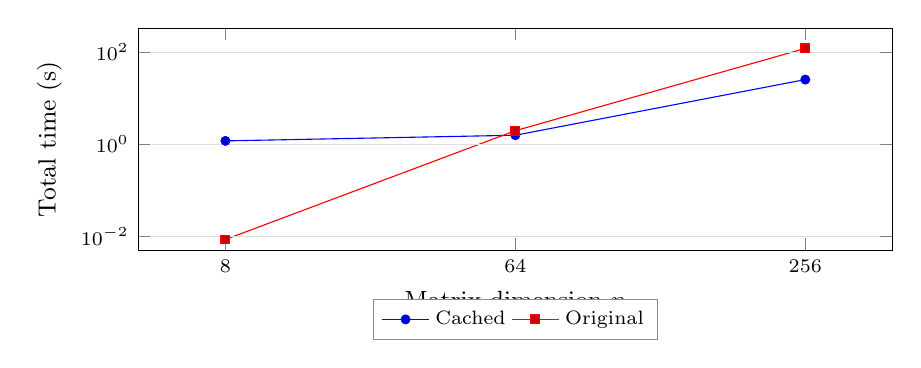
\begin{tikzpicture}
\begin{axis}[
  ieee lines,
  ymode=log,
  ymin=0.005,
  ylabel={Total time (s)},
  xlabel={Matrix dimension \(n\)},
  symbolic x coords={8,64,256},
]
\addplot coordinates {(8,1.179) (64,1.563) (256,25.291)};
\addplot coordinates {(8,0.008522) (64,1.962) (256,120.142)};
\legend{Cached, Original}
\end{axis}
\end{tikzpicture}
\caption{Total runtime, including table construction. The vertical axis is logarithmic so the \(8 \times 8\) original run remains visible.}
\label{fig:runtime}
\end{figure}

Peak memory tells a different story from the published laptop figures.
The cached process sits near 159\,MB from \(n = 8\) through \(n = 64\), which is the addition and multiplication maps, and rises to 214\,MB at \(n = 512\) as the matrices grow.
The original process is about 5\,MB until the matrices matter, and 18\,MB at \(n = 256\).
On this implementation the cache adds memory.
It does not shrink the matrices.
Figure~\ref{fig:memory} shows the sizes that both builds ran.

\begin{figure}[!t]
\centering
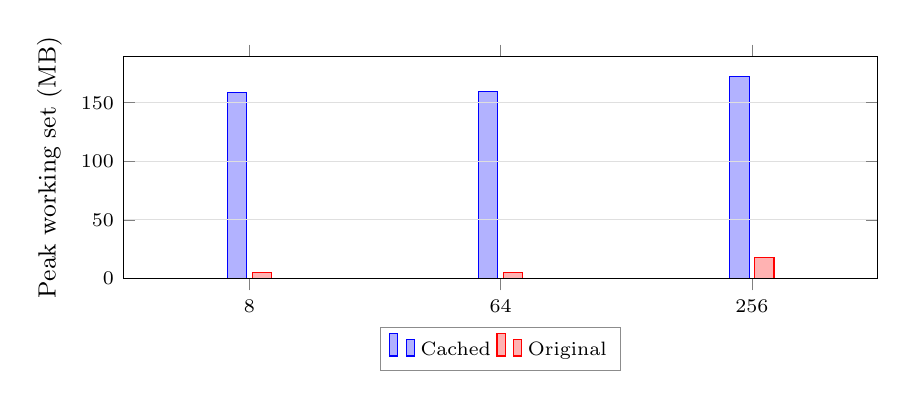
\begin{tikzpicture}
\begin{axis}[
  ieee bars,
  ymin=0,
  ylabel={Peak working set (MB)},
  xlabel={Matrix dimension \(n\)},
  symbolic x coords={8,64,256},
]
\addplot coordinates {(8,158.57) (64,159.43) (256,172.26)};
\addplot coordinates {(8,4.85) (64,5.35) (256,18.18)};
\legend{Cached, Original}
\end{axis}
\end{tikzpicture}
\caption{Peak working set on the same runs as Fig.~\ref{fig:runtime}.}
\label{fig:memory}
\end{figure}

Extending the cached \(n^3\) trend from the 194\,s run at \(n = 512\) puts a \(4000 \times 4000\) cached run near 26 hours on this CPU.
The same extrapolation of the original \(n = 256\) run puts the uncached \(4000 \times 4000\) case near 127 hours.
The assignment notes of about 20 minutes cached and 6 hours 40 minutes original were measured on an Apple M3 Max \cite{russell2026assignment}.
Those notes are a different machine and a different table layout.
They are not a prediction for the map-based tables timed here.

\section{MPI Determinant}
\label{sec:mpi}

\section{MPI Measurements}
\label{sec:mpi-results}

The MPI timings used Nicholas Johnson's branch \texttt{feature/mpi-block-plu} at commit \texttt{12b7cd3}, cloned directly because that branch was not yet merged into the group \texttt{main}.
The field dependency on that branch is the same cached fork used in Section~\ref{sec:results}.
Jobs were submitted with \texttt{sbatch} to the course cluster's Slurm partition \texttt{demo}.
That partition allows 5 minutes and has four machines, with two CPUs on each.
The MPI library is OpenMPI, loaded on the compute nodes.
The block size was 32 for every run.
Sequential mode launches one rank and uses the one-rank elimination.
The eight-rank mode places two ranks on each of the four machines.
The driver still forms \(C = AB\) on rank 0 before the determinants, so the product time is almost the same in both modes.
A run is accepted when \(\det(C) = \det(A)\det(B)\).
That check passed for every size in Table~\ref{tab:mpi}.
At \(n = 512\) the three determinants printed by the sequential run and by the eight-rank run were the same field elements.

\begin{table}[!t]
\caption{Cached sequential time against eight MPI ranks on four machines. Determinant time is the sum of \(\det(A)\), \(\det(B)\), and \(\det(C)\).}
\label{tab:mpi}
\centering
\scriptsize
\begin{tabular}{@{}rrrrr@{}}
\toprule
\(n\) & Seq. (s) & 8 ranks (s) & Seq. dets (s) & 8-rank dets (s) \\
\midrule
64  & 1.76 & 2.61 & 0.25 & 0.21 \\
128 & 5.53 & 5.61 & 2.04 & 1.09 \\
256 & 35.0 & 27.4 & 15.6 & 5.66 \\
512 & 272  & 200  & 120  & 33.5 \\
\bottomrule
\end{tabular}
\end{table}

Eight ranks are already slightly faster on the determinants at \(n = 64\), 0.21\,s against 0.25\,s.
The whole program is still slower there, 2.61\,s against 1.76\,s, because the table fill and the sequential product are larger than the determinant savings.
At \(n = 128\) the determinants drop from 2.04\,s to 1.09\,s, while the whole program is essentially tied, 5.61\,s against 5.53\,s.
The smallest tested size at which the whole program is faster with eight ranks is \(n = 256\), 27.4\,s against 35.0\,s.
At \(n = 512\) the determinant portion falls from 120\,s to 33.5\,s, a factor of about 3.6 on eight ranks, and the whole program falls from 272\,s to 200\,s.
The product at that size is still about 151\,s sequential and 164\,s with eight ranks, so most of the remaining time is work this MPI code does not divide.
Figure~\ref{fig:mpi} plots the determinant column of Table~\ref{tab:mpi}.

\begin{figure}[!t]
\centering
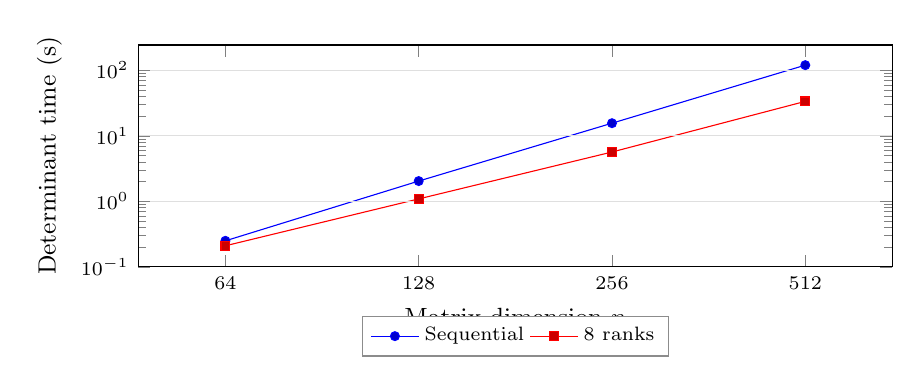
\begin{tikzpicture}
\begin{axis}[
  ieee lines,
  ymode=log,
  ymin=0.1,
  ylabel={Determinant time (s)},
  xlabel={Matrix dimension \(n\)},
  symbolic x coords={64,128,256,512},
]
\addplot coordinates {(64,0.25) (128,2.04) (256,15.58) (512,119.70)};
\addplot coordinates {(64,0.21) (128,1.09) (256,5.66) (512,33.53)};
\legend{Sequential, 8 ranks}
\end{axis}
\end{tikzpicture}
\caption{Sum of the three determinant calls on the four-machine cluster. The vertical axis is logarithmic.}
\label{fig:mpi}
\end{figure}

A second sweep used two ranks on one machine, at \(n \in \{64, 128, 256\}\), with the same block size and the same cached field.
The determinant sums were 0.23\,s against 0.23\,s at \(n = 64\), 1.91\,s against 1.61\,s at \(n = 128\), and 15.9\,s against 12.6\,s at \(n = 256\).
The whole program was faster with two ranks only at \(n = 256\), 33.9\,s against 35.6\,s.
Two ranks therefore reach a whole-program win at the same tested size as eight ranks, but the determinant speedup is smaller.
The identity check passed on that sweep as well.

The cluster could not host a larger size.
The \(512 \times 512\) sequential run took 272\,s of a 300\,s job.
An attempt to follow it with the eight-rank run in the same job was cancelled at the time limit.
The eight-rank \(512 \times 512\) numbers in Table~\ref{tab:mpi} come from a separate job that ran only that mode.
The step from 35\,s at \(n = 256\) to 272\,s at \(n = 512\) is a factor of 7.8, against the factor of 8 predicted by \(n^3\).
Applying another factor of \((4000/512)^3 \approx 477\) to the 272\,s measurement puts a cached sequential \(4000 \times 4000\) run near 36 hours on these cluster CPUs.
That case was not run.
The assignment's 20-minute cached figure remains the Apple M3 Max note, measured on a different implementation and a different computer.

\section{Conclusions}
\label{sec:conclusions}

The cached class is \texttt{FiniteFieldElement}, the element type of \texttt{FiniteField<11, 3>} at the bottom of the dependency chain.
Every matrix operation in the program reduces to sums, products, and reciprocals of these elements, so caching them speeds up the product and all three determinants at once.
The cached version keeps the original interface.
The driver and the matrix library switch between the two fields by changing one CMake dependency and nothing else.

Caching made the arithmetic about five times faster on one thread.
The tables cost about 1.2\,s to build, so the cached field loses on very small matrices and is faster in total from \(n = 64\) upward.
At \(n = 512\) the total time fell from 976\,s to 194\,s.
Both fields scale close to \(n^3\), so the gap holds at larger sizes.

Memory went the other way.
The addition and multiplication tables hold about 1.77 million entries each, which sets a floor of about 159\,MB against about 5\,MB for the original field.
At \(n = 512\) the cached run peaked at 214\,MB against 60\,MB.
The assignment's reference figures show a cached field using less memory than the original.
This implementation does not, because the matrices still store each element as a polynomial and the tables are added on top.
Storing each matrix entry as its table index would shrink the matrices as well, and is the clearest next step.

The blocked PLU determinant over MPI was faster than the cached sequential determinant at \(n = 64\), the smallest size tested.
The margin there is small, 0.071\,s against 0.078\,s, and the advantage grows to 4.0 times at \(n = 768\).
For the complete program the break-even point is \(n = 256\), because the matrix product stays on rank 0.
Rank 0 also owns every matrix and sends the trailing submatrix out and back for each panel.
Distributing ownership of the rows, and parallelizing the product, would move both break-even points down.

The \(4000 \times 4000\) case was not run on either machine.
On the PC it would take about a day, and the cluster partition allows only five minutes per job, so the reference timings remain the only figures at that size.
The PC and cluster measurements also come from different hardware and should not be compared directly.
Within those limits, the results follow the assignment's order of work: caching the expensive arithmetic gave the largest single improvement, and MPI added a further speedup once the matrices were large enough to outweigh the communication.

\section{Additional Contribution}
\label{sec:additional}

\writer{Fernanda Gonzalez}{%
This section is a placeholder because the author list includes you and no part above is assigned to you.
Replace it with your contribution, or remove this section and your name from the author list if you are not on this assignment.}


\end{document}
